%&LaTeX

\section{More Feedforward Filters}

This lab discusses the different ways in which to express a discrete
feedforward filter. When completed you should feel comfortable
representing a filter in any of its equivalent forms and know the
different advantages of expressing a filter in these forms.  When you
get down to it, feedforward filters can be expressed in the following
equivalent ways:
\begin{enumerate}
\item Defining equation, $y[n]$ as a (linear) function of $x[n],
  x[n-1], \ldots$, or equivalently as this equation's coefficients.
  % \item Impulse response, $h[n]$.
\item Transfer function, $H(z)$.
\item Frequency response (i.e., the expression for $\mathcal{H}(\hat{\omega})$). 
\item Zero locations, $z_i$, often plotted in the complex plane.
\item Amplitude $|\mathcal{H}(\hat{\omega})| = |H(e^{j\hat{\omega}})|$ (and phase
  $\theta(\hat{\omega})$) of the frequency response, often plotted as
  functions of $\hat{\omega}$.
\item Block diagram.
\end{enumerate}

In this lab, you will be given a number of filters, each expressed in
one of the above ways, for each, you are asked to generate the other
representations using pencil and paper. For our purposes here, it will
only be necessary to sketch the amplitude of the filter's frequency
response (for item 5 above).  For items 4 and 5, please use J-DSP to
check your answers. If there is disagreement between your answers and
what you get in J-DSP, please spend some time out of class discussing
the discrepancy with your classmates or with me to determine its
source.

\paragraph{Step 1: Three-point averager} Yes, we've done some of this already,
	so it's a good, familiar place to start. The defining equation is
	$y[n] = \frac{1}{3}x[n] + \frac{1}{3}x[n-1] + \frac{1}{3}x[n-2]$;
	determine the other representations.
	

\paragraph{Step 2: First-difference filter} A \emph{first-difference} filter is an
	approximation to a discrete derivative operation. Its transfer
	function is $H(z) = 1 - z^{-1}$. Determine the other representations.

	
\paragraph{Step 3: Second-difference filter} Just as we can compute a discrete
	first derivative with a first-difference filter, we can compute a
	discrete second derivative with a \emph{second difference filter}. Its
	block diagram (in a little trickier format) is:
	
	\centerline{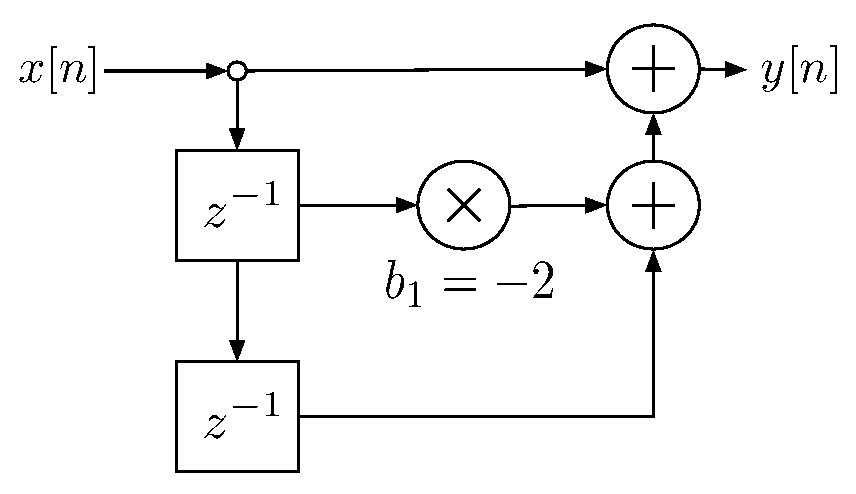
\includegraphics[width=2.5in]{lab5/second-difference-bdiag}}
	
	After you've developed the alternative representations, show that
	this filter can also be implemented as a cascade of two
	first-difference filters.
	
\paragraph{Step 4: Complex conjugate zeros} Feedforward filters with real
	coefficients in their defining equations have either real or complex
	conjugate zeros. Re-represent the filter with zeros $z_{1,2} = 0.5 \pm
	j 0.5$ and $z_3 = 0.75$.

\paragraph{Step 5: Symmetric filters} Feedforward filters with
        symmetric coefficients have interesting properties, such as
        linear phase terms. Even symmetric filters have a midpoint
        around which they mirror their coefficients. Re-represent the
        filter with a coefficients given by $\{1,2,2,1\}$ (i.e.,
        $y[n]=x[n]+2x[n-1]+2x[n-2]+x[n-3]$). In this filter, the
        coefficients \{1,2\} are mirrored.


%%% Local Variables: 
%%% mode: latex
%%% TeX-master: t
%%% End: 
